Recall the 1D steady-state heat equation with constant diffusivity over the interval $[0,1]$
\begin{align*}
-\pd{u}{x}{2} &= f\\
u(0) &= u(1) = 0.
\end{align*}
Recall from class the finite difference approximation to this problem: given a set of points $x_0,\ldots, x_{N+1}$, solved for the solution $u(x_i)$ at each point by approximating $\pd[2]{u}{x}$ with
\[
u''({x_i}) \approx \frac{u(x_{i-1}) - 2u(x_i) + u(x_{i+1})}{h^2}, \quad i = 1,\ldots, N
\]
(where $h$ is the spacing between points $x_{i+1}$ and $x_i$) along with the conditions that
\[
u(x_0) = u(x_{N+1}) = 0.
\]

We will modify this finite difference approximation to accomodate instead the Neumann boundary condition of $u'(1) = 0$ at $x=1$.
\begin{enumerate}
\item We would like to enforce that $u'(x_{N+1}) = 0$, but if we approximate $u'(x_{N+1})$ with a central difference
\[
u'(x_{N+1}) \approx \frac{u(x_{N+\frac{3}{2}})-u(x_{N+\frac{1}{2}})}{h},
\]
we end up with an equation involving $u(x_{N+\frac{3}{2}})$, which does not lie inside the interval $[0,1]$. Instead, we can define a \textit{backward difference} approximation to the derivative
\[
u'(x_{N+1}) \approx \frac{u(x_{N+1})-u(x_N)}{h} = 0
\]
and set this to zero instead. Write out the expression for $u''(x_N)$ in terms of $u(x_i)$ and use the backward difference approximation for $u'(x_{N+1})$ to eliminate $u(x_{N+1})$.
\item Determine the exact solution to $-u''(x) = 1$ for $u(0) = 0$, $u'(1) = 0$ (hint: the solution is a quadratic function).
\item Create a \textsc{Matlab} script that constructs the matrix system $Au = f$ resulting from the finite difference equations when $f = 1$.  Plot the computed solution values $u(x_i)$, as well as the error at each point $|u_{\rm exact}(x_i)-u(x_i)|$, for $i = 0,\ldots, N+1$ for $N = 16, 32, 64, 128$, and label each appropriately.  Where is the error largest?
%\item Suppose we have $u'(0) = u'(1) = 0$. Show that if $u(x)$ is a solution of the steady state heat equation with these boundary conditions, that
%\[
%u + C
%\]
%for any constant $C$ is also a solution to the same steady state heat equation. This shows that there is no \textit{unique} solution to the steady state heat equation under these boundary conditions.
%\item Construct the finite difference equations as in part (b), but for the boundary conditions $u'(0) = u'(1) = 1$. Since the heat equation does not have a unique solution, we do not expect the finite difference system to have one either. How does this show up in the matrix equations that result from the finite difference approximation?
\end{enumerate}


%%%%%%%%%%%%%%%%%%%%%%%%%%%%%%%%%%%%%%%%%%%%%%%%%%%%%%%%%%%%

\ifthenelse{\boolean{showsols}}{

\begin{solution}
\begin{enumerate}
\item We can rewrite the finite difference approximation to $-u''(x) = f(x)$ at point $x_N$ as
\[
-\frac{u(x_{N-1}) - 2u(x_N) + u(x_{N+1})}{h^2} = f(x_N).
\]
Note that
\[
\frac{u(x_{N-1}) - 2u(x_N) + u(x_{N+1})}{h^2} = \frac{u(x_{N-1}) - u(x_N)}{h^2} + \frac{u(x_{N+1})-u(x_N)}{h^2}
\]
Using the backwards difference approximation to $u'(x_{N+1})$, we have
\[
\frac{u(x_{N+1})-u(x_N)}{h^2} = 0
\]
which simplifies our finite difference equation at $x_N$ to
\[
-\frac{u(x_{N-1}) - u(x_N)}{h^2} = f(x_N).
\]
(Note that the boundary condition also implies $x_N = x_{N+1}$).
\item We can integrate the differential equation twice to get the boundary conditions.
\[
\int_0^x -u''(s)ds = \int_0^x 1 ds
\]
where $s$ is a dummy variable for integration. By the fundamental theorem of calculus, this gives
\[
-u'(x) + u'(0) = x.
\]
Since we don't know the value of $u'(0)$, we consider it an unknown constant $C_1$ that we have to determine using our boundary conditions. Repeating the process again gives
\[
\int_0^x(-u'(s) + C_1) ds = \int_0^x x ds
\]
which results in
\[
-u(x) + C_1x + u(0) = \frac{x^2}{2}.
\]
We could set $u(0)$ to be a constant $C_2$ to be determined by the boundary conditions as well; however, since we know $u(0) = 0$ from the boundary conditions, we can go ahead and zero it out.

The end result gives
\[
u(x) = -\frac{x^2}{2} + C_1x
\]
The above form of the equation and the boundary condition $u'(1) = 0$ give the condition that
\[
u'(1) = -1 + C_1 = 0
\]
implying $C_1 = 1$, and
\[
u(x) = -\frac{x^2}{2} + x = \frac{1}{2}x(2-x).
\]

Alternatively, since the problem specifies the solution is a quadratic, it is possible to simply specify
\[
u(x) = ax^2 + bx + c
\]
and use the differential equation and boundary conditions to determine the constants.
\item Since the finite difference equations must be satisfied at each point $x_i$, they lead to a series of $N$ equations with $N$ unknowns (the values of $u(x_i)$ for $i = 1,\ldots, N$).
The matrix system resulting from these equations for homogeneous boundary conditions
\[
u(0) = u(1) = 0
\]
is
\[
{-1\over h^2} \left[\begin{array}{rrrr}
              -2 & 1 \\[0.25em]
               1 & -2 & 1 \\
                 &  1  & -2 & \ddots \\
                 & & \ddots & \ddots & 1 \\[0.25em]
                 & & & 1 & -2
               \end{array}\right]
          \left[\begin{array}{c} u_1 \\[0.25em] u_2 \\[0.25em] \vdots \\[0.25em] u_{N-1} \\[0.25em] u_N \end{array}\right]
 =   \left[\begin{array}{c} f(x_1) \\[0.25em] f(x_2) \\[0.25em] \vdots \\[0.25em] f(x_{N-1}) \\[0.25em] f(x_N) \end{array}\right],
\]
where $u_i \approx u(x_i)$. Since we have the boundary condition $u'(1) = 0$ instead, this changes our finite difference equation at point $x_N$, which corresponds to the final row of our matrix. Thus, our new matrix system for a no-flux boundary condition at $x = 1$ will be
\[
{-1\over h^2} \left[\begin{array}{rrrrr}
              -2 & 1 \\[0.25em]
               1 & -2 & 1 \\
                 &  1  & -2 & \ddots \\
                 & & \ddots & \ddots & 1 \\[0.25em]
                 & & & 1 & -1
               \end{array}\right]
          \left[\begin{array}{c} u_1 \\[0.25em] u_2 \\[0.25em] \vdots \\[0.25em] u_{N-1} \\[0.25em] u_N \end{array}\right]
 =   \left[\begin{array}{c} f(x_1) \\[0.25em] f(x_2) \\[0.25em] \vdots \\[0.25em] f(x_{N-1}) \\[0.25em] f(x_N) \end{array}\right].
\]
Included is Matlab code that can be used to generate the finite difference solution and the error between it and the exact solution:
\lstinputlisting{hw1_p4.m}
\begin{figure}
\centering
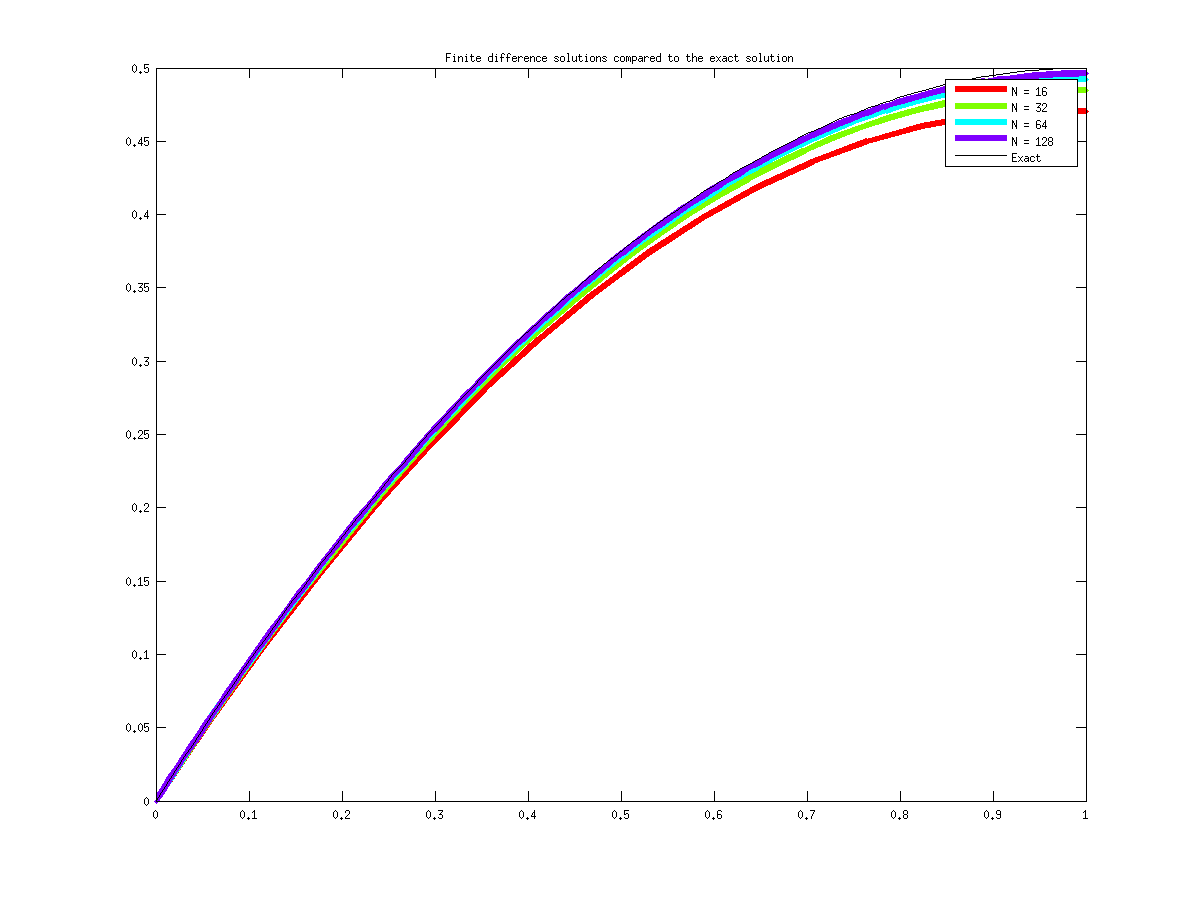
\includegraphics[width=.8\textwidth]{p4c_sol.png}
\caption{Finite difference solutions for various $N$}
\end{figure}
\begin{figure}
\centering
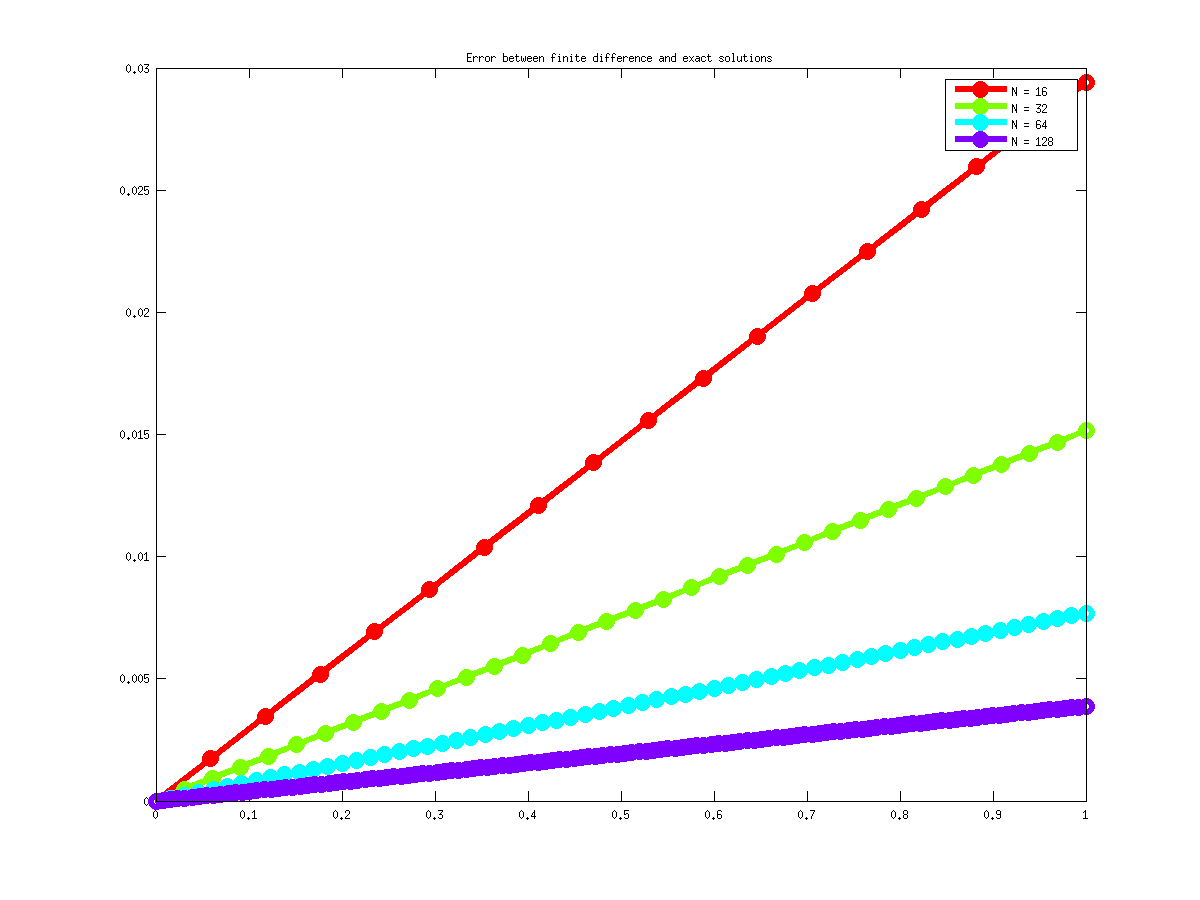
\includegraphics[width=.8\textwidth]{p4c_error.png}
\caption{Error between the exact solution and finite difference solution at points $x_i$.}
\end{figure}
\item If $u(x)$ is a solution, then $u(x)$ satisfies $u'(0) = u'(1) = 0$ and that
\[
-u''(x) = f.
\]
Then, notice that $u + C$ also satisfies the same differential equation: $(u+C)'(x) = (u'+C')(x) = u'(x)$, since $C$ is constant. Thus, the boundary conditions are satisfied. Taking two derivatives of $(u+C)''(x) = u''(x)$ for the same reason, which implies that $u+C$ also satisfies the differential equation.
\end{enumerate}
\end{solution}
}

